\chapter{Conclusion}\label{conclusion}
 
\section{Summary}
The goal of this work has been to develop novel methods of increasing the generalizability of deep learning models, as well as to survey the relative impacts of more conventional components of the deep learning pipeline. This was achieved as follows:

\Cref{background} provided an overview of deep learning, segmentation, and delved further into why such systems so readily fail to generalize, starting from first principles and analyzing the shortcomings of \gls{erm}. This was then connected to recent analyses of generalizability failure, including the notion of underspecification and shortcut learning. Finally, known methods of increasing generalization as presented in EndoCV2021 and elsewhere in the literature were then discussed and analyzed with respect to the established theory. 

This was then in turn used to inform the development of the methods discussed in~\Cref{methods}, including a novel training paradigm, augmentation technique, model architecture and ensemble models. Each of these methods were also discussed with respect to the theory explored in~\Cref{background}.

Several experiments were then conducted in~\Cref{experiments} in order to ascertain the impact of the proposed methods:
First, baseline generalizability metric were collected for five separate models. The findings supported the notion that larger models are more prone to generalizability failure, as demonstrated by the significant gap between the Unet and the TriUnet. The use of a secondary decoder in the DD-DeepLabV3+ model was shown to have negligible impact, despite reducing performance variability. It was hypothesized that this is due to the encoder already learning domain- and dataset-independent features. 

In the next experiment, data augmentation was shown to increase generalizability by a considerable margin. Synthetic augmentation via inpainting was shown to hamper this improvement when used in conjunction with regular augmentation, but this finding was deemed inconclusive due to the relatively low performance of the inpainter. 
The impact of Consistency Training was then tested and compared to regular data augmentation and no augmentation. The results show that Consistency Training outperforms regular data augmentation by a considerable margin on the most difficult of the three \gls{ood} datasets. 

Finally, predictors trained according to the best methods as identified in the previous experiments were then combined into ensembles. The results demonstrated the generalizability of ensemble-based methods, but further analysis did not sufficiently corroborate that this improvement can be attributed to ensembles mitigating underspecification. 

The results from this experiment was then discussed in~\Cref{discussion}. Limitations of the experiments were noted, along with their practical impacts and possible directions of further study and potential ways to improve the methods proposed in this thesis. 


\section{Contributions}
The main contributions in this thesis can be regarded as twofold:

First, the thesis introduced a number of novel methods intended to increase generalization, most notably a new way of thinking about generalization as consistency to perturbations. This informed the development of Consistency Training, which was shown to increase generalizability by a considerable margin, serving as a more generalizable alternative to data augmentation. This framework, and the potential improvements that can be made upon it as suggested in~\Cref{discussion}, shows good promise with regards to further increasing generalizability. The ensemble models consisting of predictors according to Consistency Training was also shown to increase generalization. Though the remaining methods - i.e generative inpainting and DD-DeepLabV3+ - were proven ineffective, the analysis thereof nevertheless motivated a number of directions of further study. 


Second, this work provides an quantitative analysis  of how generalizability is affected by the choice of model architecture, augmentation strategy, and the use of ensembles. Though most of the findings corroborated the literature, there were a fair number of surprising results that warrant further investigation, in particular with regards to the impacts of the tested methods relative to one another. For one, the effect of multitask learning and generally the the choice of model architecture was practically negligible. With the exception of TriUnet, every tested model exhibited practically identical performance. Ensembles, though exhibiting statistically significant impact, resulted in somewhat marginal improvements on generalization, especially in comparison to the use of data augmentation and Consistency Training. As discussed in~\Cref{discussion}, this raises doubts as to the veracity of findings in other literature, where data augmentation is rarely accounted for when performing comparisons. Hopefully, the findings in this thesis demonstrates the need for a more structured approach to the design of experimental methodologies intended to analyze generalization, wherein the constituent components of the pipeline are sufficiently controlled. 


\section{Future work} \label{future_work}
  In addition to further developing and analyzing the methods presented in this thesis, some ideas for which were presented in~\Cref{discussion}, there are several directions of future research that may provide further insight into generalizability and generalization failure. This section will cover a number of these ideas. 
    \subsection{Deep Preprocessing} \label{denoising}
        In Consistency Training, the objective is to optimize for features that are consistent across perturbations such that the model learns invariance to distributional shifts that should not affect the causal structure of the problem. Though this as established increases generalizability, it may also be possible to simply preprocess the images such that \gls{ood} transformations or artifacts are accounted for. This is achieved elsewhere in the literature using generative models - for instance a CycleGAN~\cite{cyclegan}, which maps the input data between domains prior to being given to the segmentation network. One could implement a similar system using Consistency Training through the use of a denoising network. The resulting pipeline is illustrated in~\Cref{fig:preproc}.
        
        \begin{figure}[htb]
            \centering
           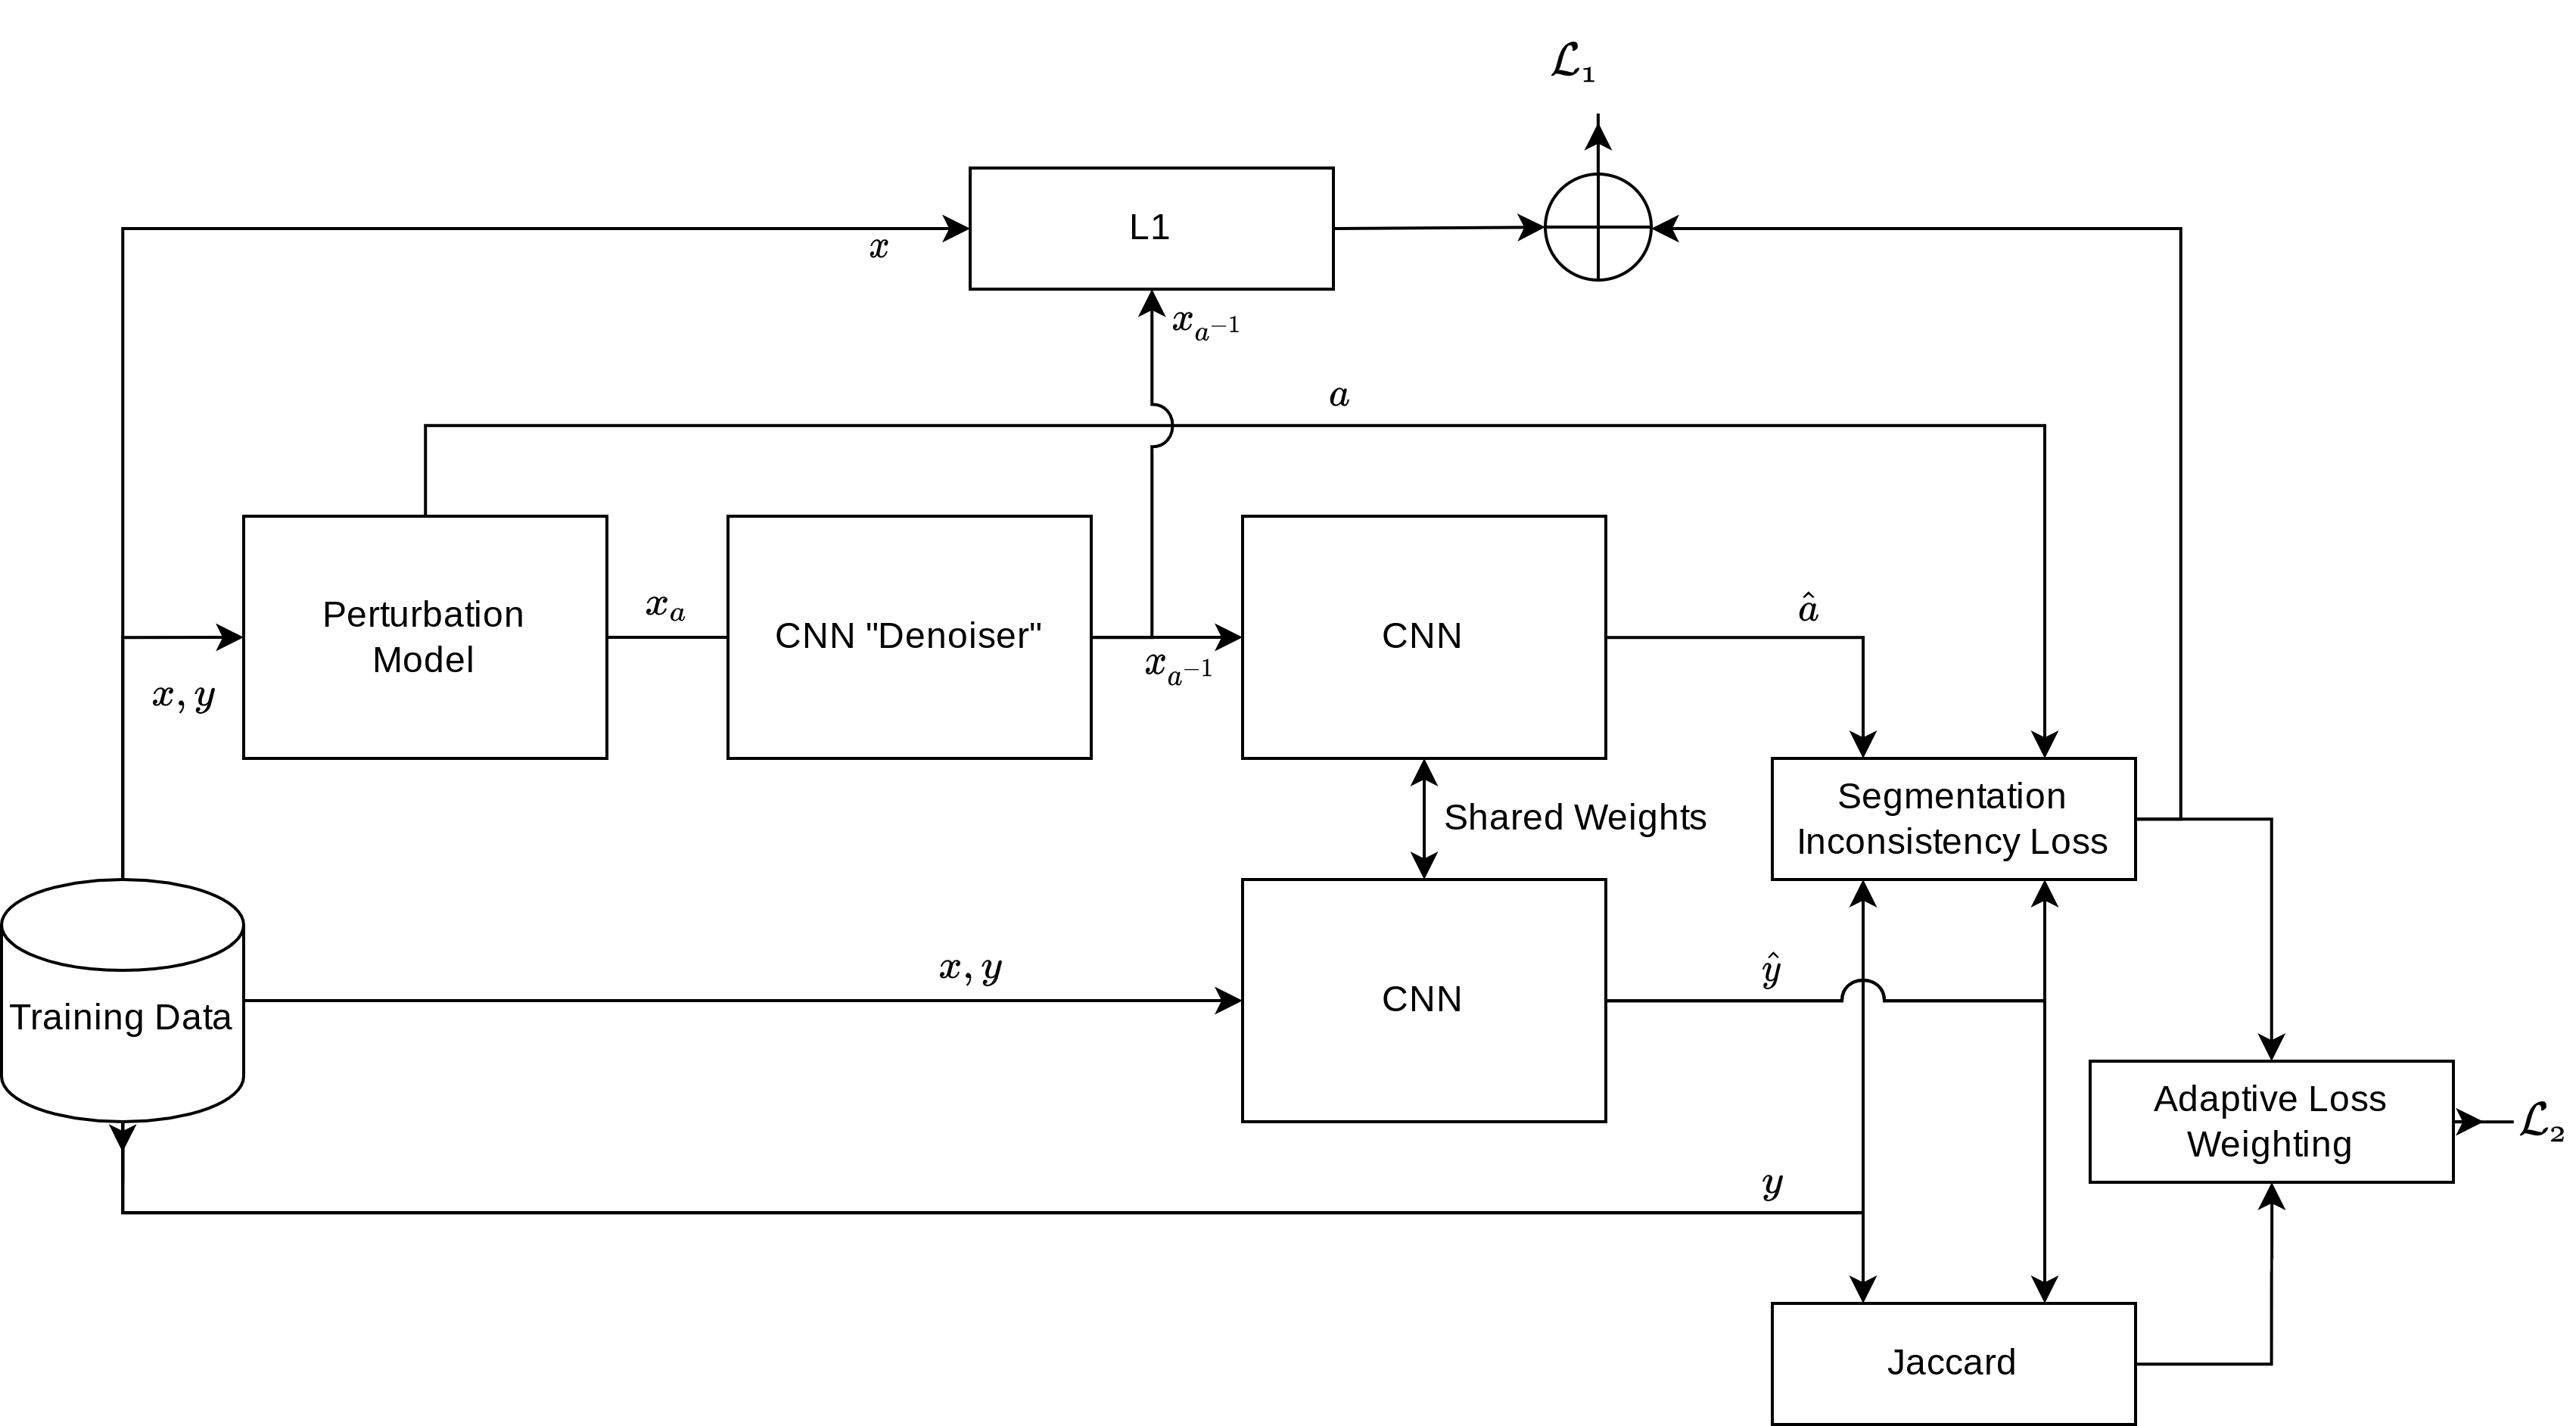
\includegraphics[width=\linewidth]{illustrations/deep_preprocessing.png}
            \caption{Consistency Preprocessing Pipeline}
            \label{fig:preproc}
        \end{figure}
        
        There are two main differences between this pipelines and more conventional deep denoising pipelines. First, the segmentation models are trained using Consistency Training. Second, the denoising network is incorporating inconsistency loss as a component of the loss function. There would in this case be two separate loss functions, one for each network. In theory, this should result in the denoiser learning to counteract the characteristics of the perturbations being applied that most negatively affect the consistency and thus the generalization of the segmentation models. Moreover, even if the denoiser performs poorly, the segmentation portion should be generalizable due to Consistency Training, which may even be improved as a result of whatever transforms the denoising network is performing.
        
        
    \subsection{Further investigations of multitask learning}
        Multitask learning was only briefly investigated in this thesis through the dual-decoder DeepLabV3+, which as a reminder performed image reconstruction as an auxiliary tasks. Though this was shown to have negligible effects, which was hypothesized may be the result of segmentation encoders learning task-agnostic features - the results are by no means sufficiently conclusive to discredit multitask learning altogether. 
    
        Further investigating the impact of multitask learning on generalization is as such warranted. One could for instance perform a study on the impact of different tasks; perhaps image reconstruction is less conducive to generalization than something more task-adjacent, such as dimming the background or simple object detection. Depending on the results of this study, one could then also experiment with adding multiple auxiliary tasks. Investigating the variance of the latent representation in these models across multiple runs of training and comparing these to the variance in single-task models may be interesting and further the understanding of what \glspl{dnn} actually learn.
        
        Modifying the models to a greater extent than merely adding additional decoders would in this case also be warranted. One may for instance investigate whether the segmentation task could be decoupled into a series of multiple stages consisting of simpler tasks.
    
    \subsection{Pretraining} \label{pretraining}
        A largely neglected but nevertheless impactful aspect of the deep learning pipelines studied in this thesis is the use of pretraining. Across all the experiments performed in this thesis, every predictor was pretrained on Imagenet, with the pretrained weights being included in the segmentation-models-pytorch library~\cite{smp}. Without pretraining, the models selected in this thesis exhibited \glspl{iou} of at best around 0.6 at best even on \gls{iid}, with even more significant performance gaps on \gls{ood} data. Naturally, non-pretrained networks are for this reason rarely used. However, this pretraining may play a key role in certain aspects of the behaviour observed in this thesis. In particular, pretraining may be the principle contributing factor behind the apparent ineffectiveness of multitask learning. An Imagenet pretrained encoder would, after all, perform the best when practically performing image compression.